
\chapter{Executable Models and Simulation}

Super-languages must be expressive. Apart from language engineering,
super-languages play an important role in the design of systems by
providing a technology for building prototypes or executable models.
This chapter shows how XMF can be used to construct an executable
model of a job-shop system and then be used to perform some analysis
of the modelled system.

The simplest sketch of a system on the back of a napkin is a model
that can tell us something about the intended structure and behaviour
of the system. Models tend to fall into distinct categories that reflect
their intent. Models of usage (such as use-case models) try to capture
the client view of the system, i.e. what does the system offer? Archtecture
models try to capture the major components of the system and how they
will communicate. Data models try to capture the information that
the system processes. Dynamic models try to produce descriptions of
how the system behaves under certain conditions. In all cases, these
models may be constructed as lightweight sketches that ignore implementation
detail or constructed as detailed blueprints including key implementation
features.

To be effective, modelling must be integrated with a project development
method. There are many such methods; one significant method is to
use modelling to produce a complete executable simulation of the system.
The model is representative of the real system and is used to run
test cases. The model does not need to deal with complex implementation
details. Once the executable model has been developed and used to
analyse the behaviour of the required system, it can be used as an
executable blueprint for the real system.

There are a number of advantages to this approach: results can be
produced in a short time; requirements engineering can involve presenting
stakeholders with a simulation of the required system; the languages
used for executable modelling support good debugging and instrumentation;
the languages provide high level support for manipulating data and
representing key application components; using the executable model
as a blueprint significantly reduces the gap between design and implementation.

In order to simulate a system, a model must include the actions that
the system performs. There are a variety of ways of modelling actions
including state machines and model based action languages. Modelling
actions falls broadly into two categories that differ depending on
whether the model is to be executable or whether it is to be used
to analyse system executions. The former allows the model to be run.
The latter statically describes the properties of executions.

Section \ref{sec:A-Job-Shop-Simulation} specifies a simple job-shop
application and shows how the simulator will behave. Section \ref{sec:Job-Shop-Implementation}
describes how the simulation is implemented. Finally, section \ref{sec:Conflict-Analysis}
describes how dynamic execution behaviours can be modelled and subsequently
analysed.


\section{A Job-Shop Simulation}

\begin{figure} \begin{center}
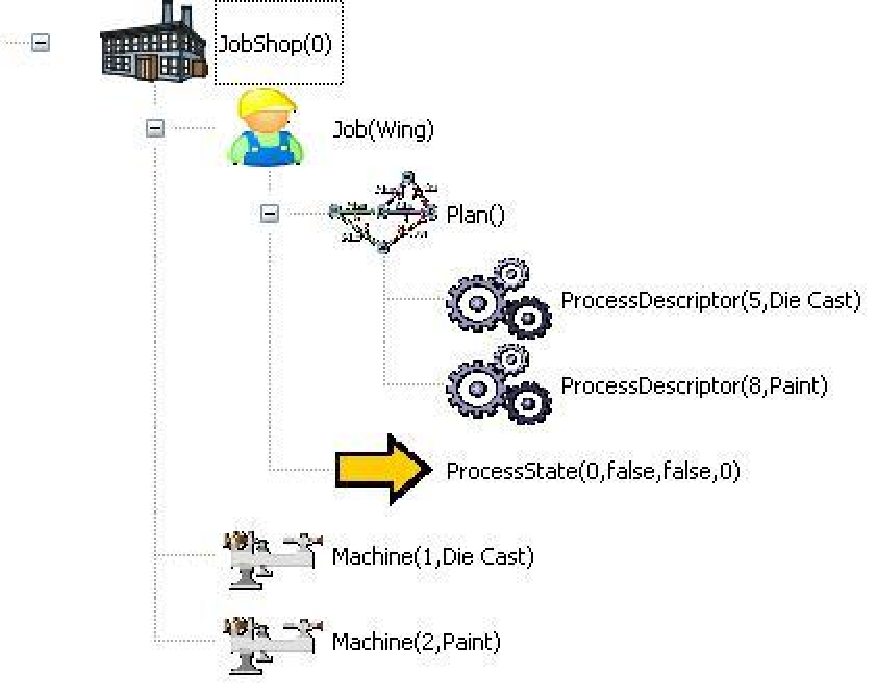
\includegraphics[width=12cm]{Programming/Simulation/Images/WingJobShop.pdf}

\caption{A Job Shop Application\label{fig:A-Job-Shop-Application}}

\end{center} \end{figure}



%
\begin{figure}
\begin{center}

\subfigure[Initial State of the Job Shop]{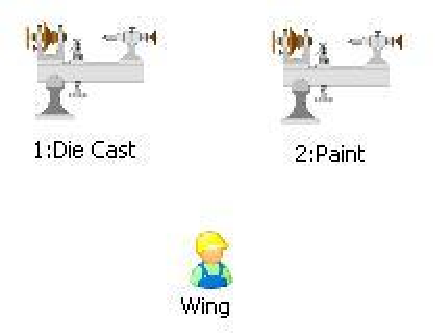
\includegraphics[width=4cm]{Programming/Simulation/Images/Wing1.pdf}}

\subfigure[Allocated to the Die Cast Machine]{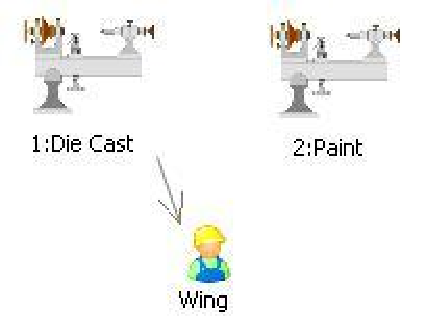
\includegraphics[width=4cm]{Programming/Simulation/Images/Wing2.pdf}}

\subfigure[Allocation to the Paint Machine]{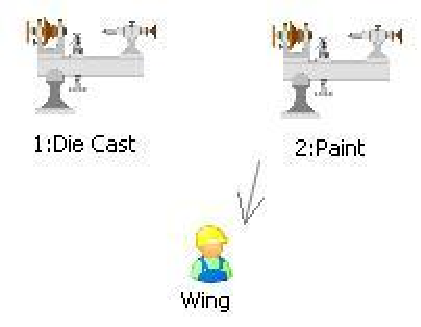
\includegraphics[width=4cm]{Programming/Simulation/Images/Wing3.pdf}}

\subfigure[Final State]{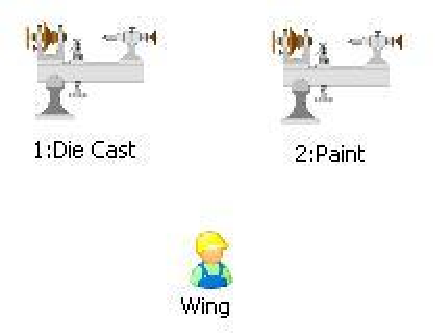
\includegraphics[width=4cm]{Programming/Simulation/Images/Wing1.pdf}}

\caption{Job Shop Simulation\label{fig:Job-Shop-Simulation-Steps}}

\end{center}
\end{figure}


Scheduling jobs is a typical example of an application that can benefit
from simulation. There are many ways in which jobs can be scheduled
to machines that process the jobs and the behaviour of a scheduling
application can change depending on many different features of the
application. Opportunistic scheduling is a simple type of scheduling
whereby jobs are allocated to machines as soon as the machine becomes
available without any fancy analysis of the best use of resources.
This section describes an executable model for opportunistic scheduling.

Figure \ref{fig:A-Job-Shop-Application} shows a simple jobs shop
as a tree of components. The job shop contains jobs that must be processed
and machines that can process the jobs. In this case the application
is to process an aircraft wing. The single job named Wing has a plan
that specifies a sequence of processes that must be performed in order.
The wing must be case by a die casting machine and then painted by
a painting machine. The job-shop has exactly one machine of each type
(therefore the task is do-able).

Figure \ref{fig:Job-Shop-Simulation-Steps} shows the steps in performing
this simple simulation. The initial state of the jobs shop shows that
the Wing job is not allocated to any machine. The job is then allocated
to the Die Case machine for 5 units of time after which is switches
to the Paint machine for 8 units of time and finally the job is complete
and not allocated to any machines.

%
\begin{figure}
\begin{center}

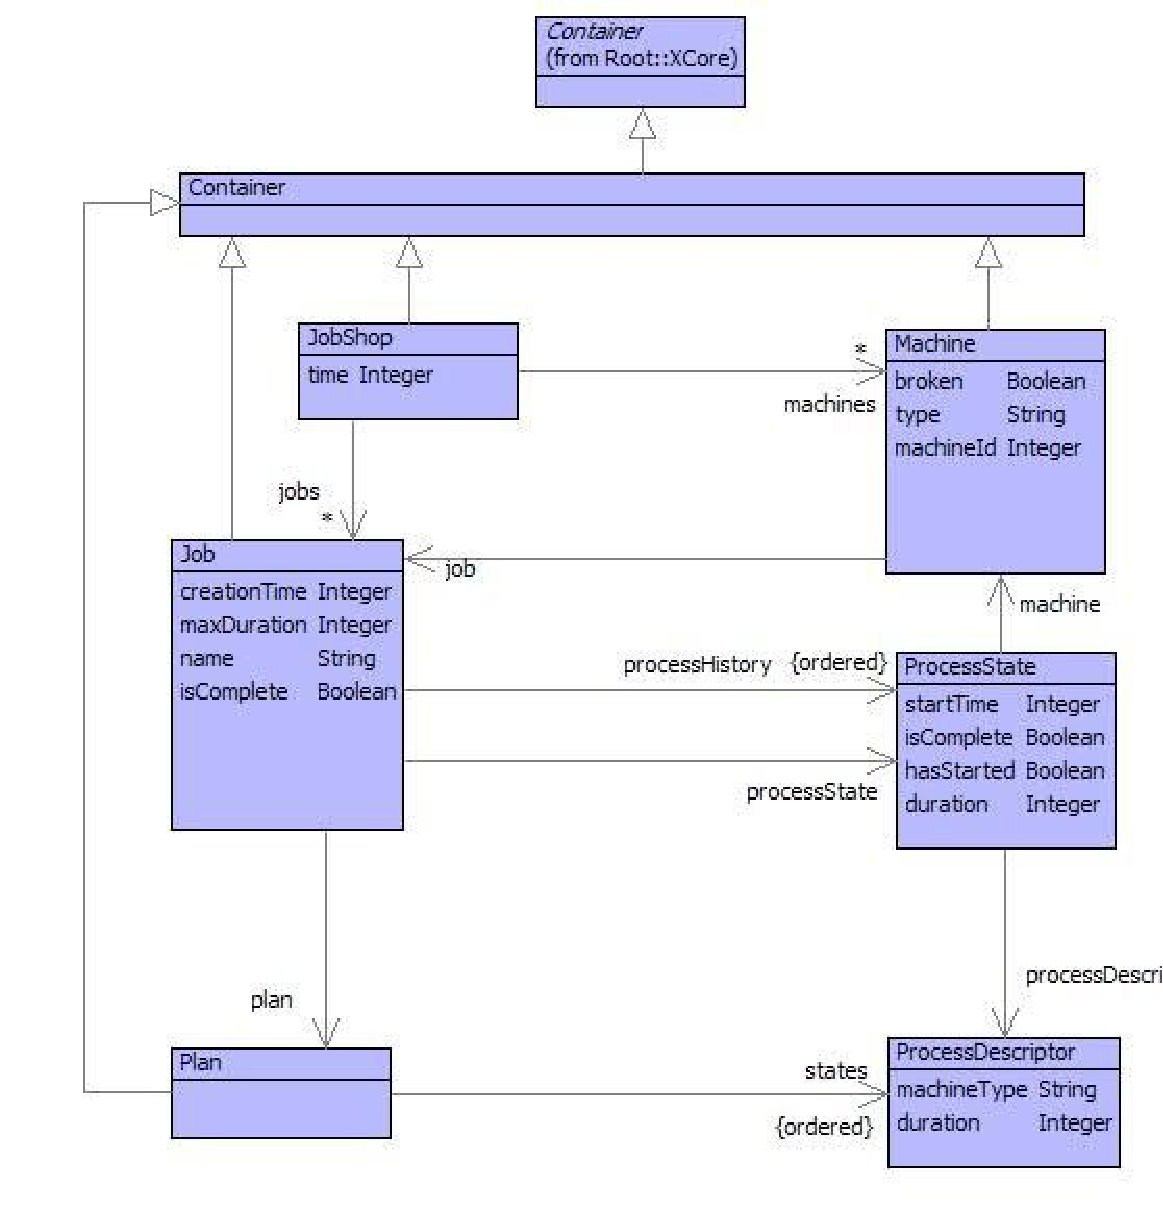
\includegraphics[width=12cm]{Programming/Simulation/Images/JobShop.pdf}

\caption{JobShop Model\label{fig:JobShop-Model}}

\end{center}
\end{figure}


Figure \ref{fig:JobShop-Model} shows a model of a job-shop consisting
of jobs to be processed and machines that can process jobs. The required
application is an opportunistic scheduler that will allocate jobs
to appropriate machines as soon as they become available. Each job
has a plan that is a sequence of process descriptors: at any given
time, a job is either completed or is waiting to be allocated to a
machine or is being processed by a machine. A machine performs processes
of a given type and can only process one job at a time. 

The model allows various configurations of machines and jobs to be
created. By attaching actions to the classes in the model it is then
possible to simulate the execution of the configuration. The results
of the simulation can be used to analyse both the configuration and
the impact of modifications to the configuration. These include: determining
the overall execution time, whether there are any bottlenecks in the
system; the effect of adding and removing machines of various types;
and, the amount of time machines are left idle.

The rest of this section describes the classes in the model in detail
and gives some example executions of the simulation. The following
section describes the implementation of the executable model.

Class JobShop records the current time and has a number of jobs and
machines. At the end of the simulation, all of the jobs are complete.
Each machine has a unique id, a type and may be broken. The type of
the machine determines the tasks that it can perform. A machine has
a current job that may be empty. If it is non-empty then the machine
is currently processing the job and the type of the machine must match
the process at the head of the job's plan. 

Class Job has a name, a creation time (allowing for jobs to be dynamically
added to the system) and a maximum allowed duration (allowing for
the simulation to determine whether a job is taking too long). A job
becomes complete when the last process in its plan is performed by
a machine. 

Each job has a plan consisting of a sequence of process descriptors.
Class ProcessDescriptor defines the machine that must perform the
processing and the length of time that the process takes. 

A job is in a current state, which may be null if it is between tasks.
If the job is being processed by a machine then the current state
has a process descriptor and a machine: the type of the machine must
match the type in the prcess descriptor.

class ProcessState records the time at which it is created. It knows
the duration that the task must take from the process descriptor and
can therefore describe when it is complete. When a task is complete,
the current state of a job is set to null, however the job has a process
history that can be used for analysis (in a real implementation a
job may not require a process history). The process history is the
sequence of all process states that the job has performed.

%
\begin{figure}
\begin{center}
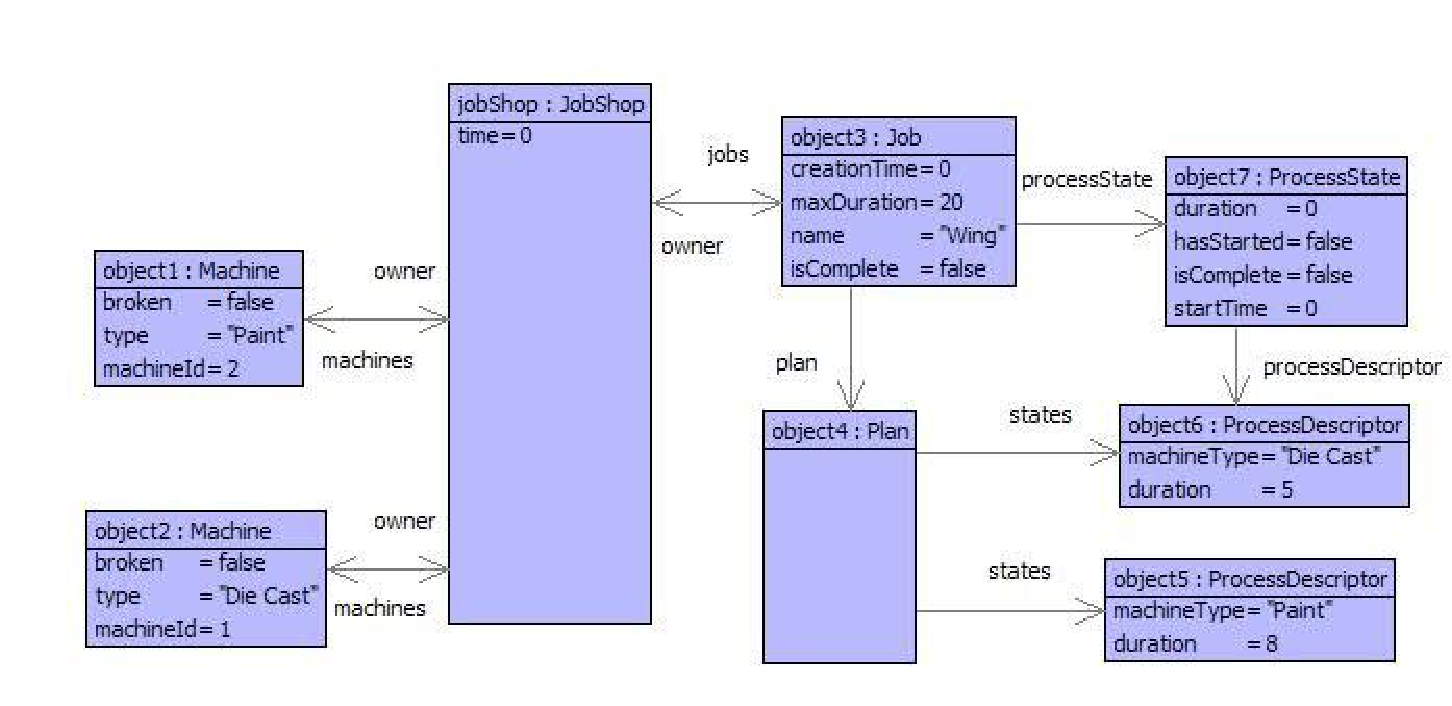
\includegraphics[width=14cm]{Programming/Simulation/Images/ProcessWing.pdf}

\caption{A Job Shop Scenario. \label{fig:Process-Wing}}

\end{center}
\end{figure}


Figure \ref{fig:Process-Wing} shows a simple initial state for a
job shop that processes aircraft wings. The job is started with an
initial process state set up for the initial process descriptor in
the plan; however, the process state shows that the process has not
started and is not yet allocated to a machine.

%
\begin{figure}
\begin{center}

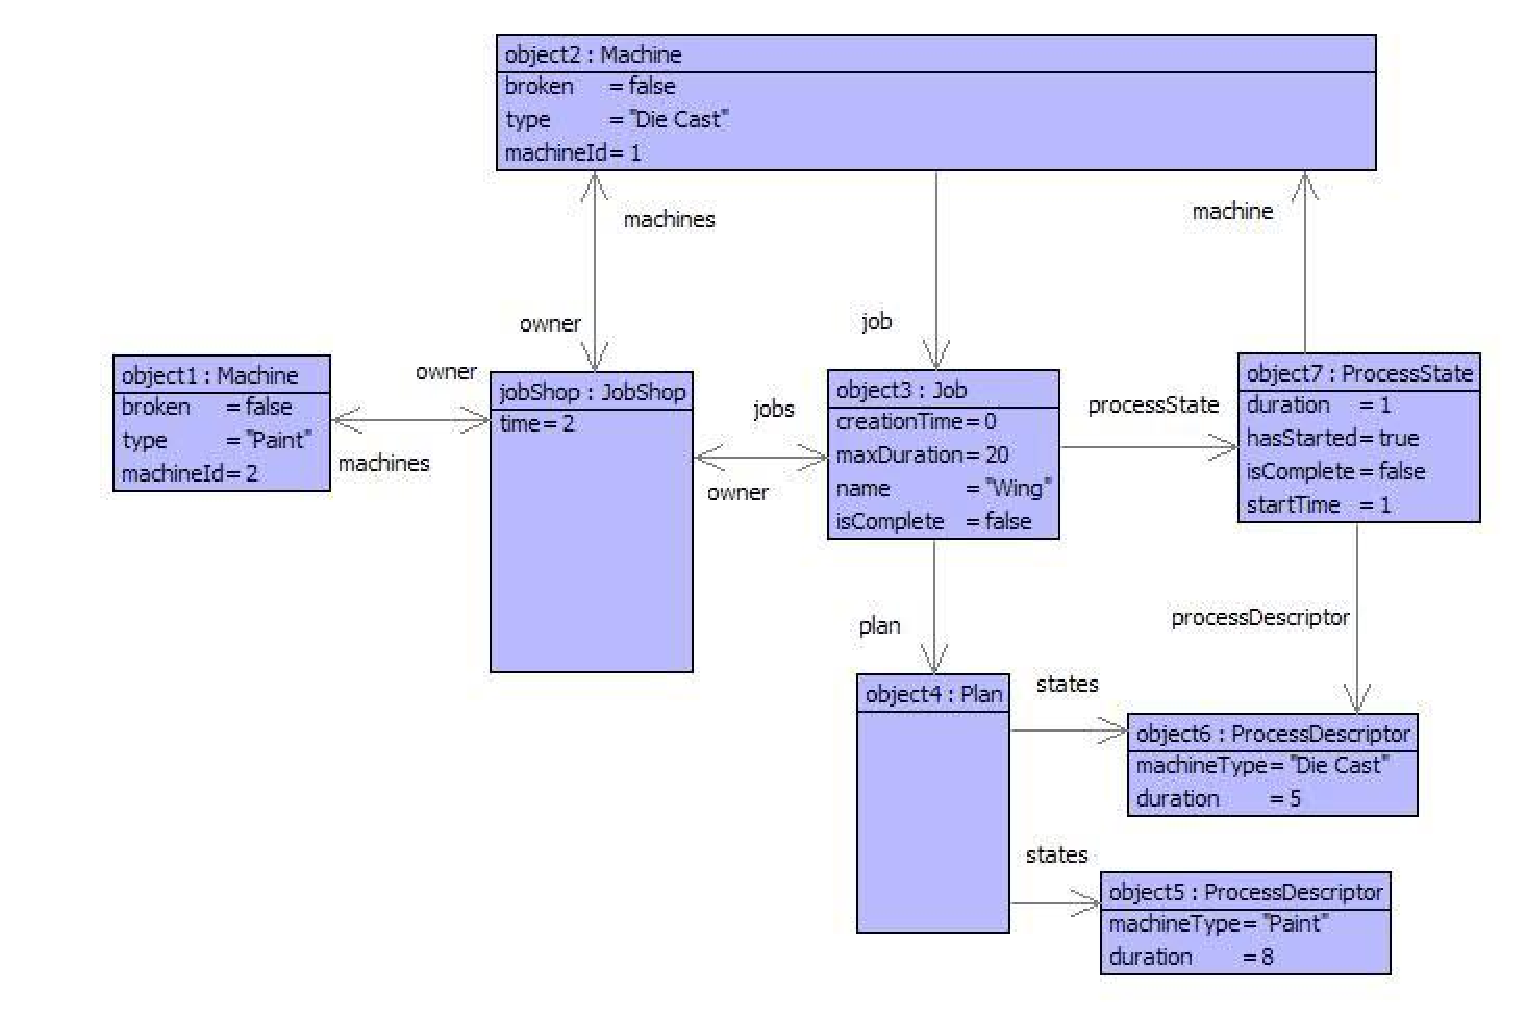
\includegraphics[width=14cm]{Programming/Simulation/Images/ProcessWing2.pdf}

\caption{At time 2 \label{fig:At-time-2}}

\end{center}
\end{figure}


Figure \ref{fig:At-time-2} shows the state of the simulator at time
2 when the initial process state has started. The process state is
allocated to a machine of the appropriate type, but is not yet complete.

%
\begin{figure}
\begin{center}

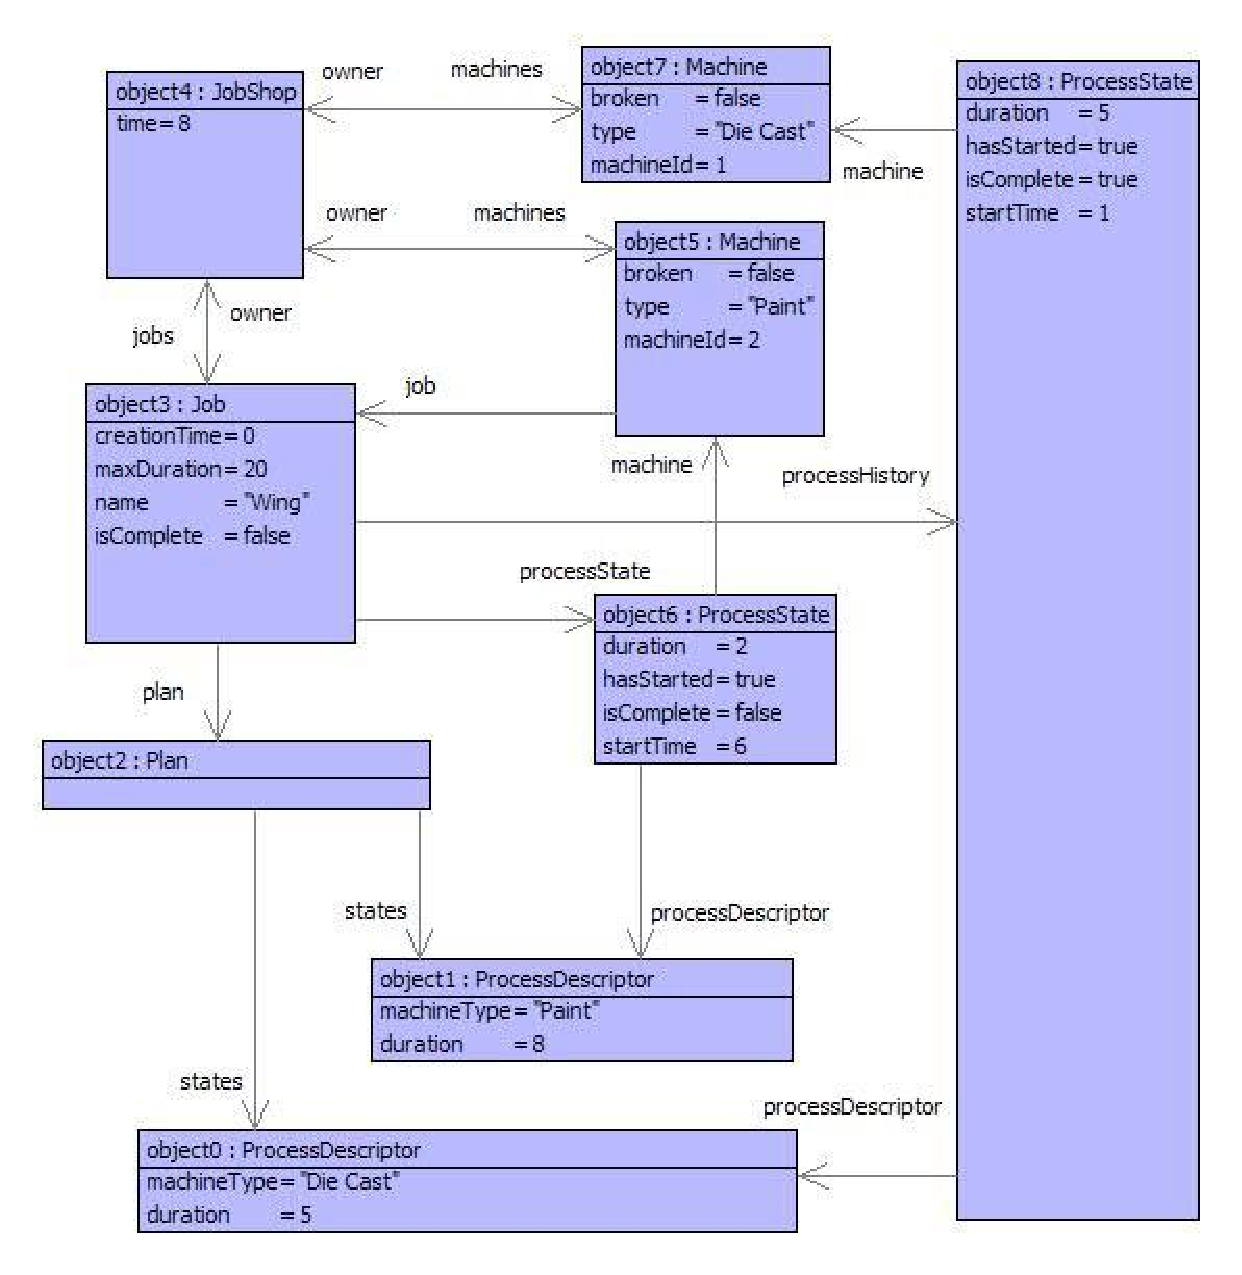
\includegraphics[width=14cm]{Programming/Simulation/Images/ProcessWing3.pdf}

\caption{After 8 time units.\label{fig:After-8-time}}

\end{center}
\end{figure}


Figure \ref{fig:After-8-time} shows the state of the simulation at
time 8. Machining at the Die Cast has completed and is shown on the
process history of the job. The process state shows that the job is
now scheduled at the paining machine. The simulation continues at
the painting machine until the time reaches 16 when the job becomes
complete.

A trace of the simulation is shown below:

\begin{lstlisting}
[1] XMF> ProcessWing::jobShop.run();
[1  ] Job Wing becomes scheduled at machine Die Cast:1.
[2  ] Machine Die Cast:1 processing job Wing (1 of 5 units)
[3  ] Machine Die Cast:1 processing job Wing (2 of 5 units)
[4  ] Machine Die Cast:1 processing job Wing (3 of 5 units)
[5  ] Machine Die Cast:1 processing job Wing (4 of 5 units)
[6  ] Machine Die Cast:1 completes job Wing.
[6  ] Job Wing becomes scheduled at machine Paint:2.
[7  ] Machine Paint:2 processing job Wing (1 of 8 units)
[8  ] Machine Paint:2 processing job Wing (2 of 8 units)
[9  ] Machine Paint:2 processing job Wing (3 of 8 units)
[10 ] Machine Paint:2 processing job Wing (4 of 8 units)
[11 ] Machine Paint:2 processing job Wing (5 of 8 units)
[12 ] Machine Paint:2 processing job Wing (6 of 8 units)
[13 ] Machine Paint:2 processing job Wing (7 of 8 units)
[14 ] Machine Paint:2 completes job Wing.
true
[1] XMF>
\end{lstlisting}Once the job shop simulation has completed, it is possible to perform
analysis on the job histories. One useful analysis is to determine
when any of the machines have been idle during the simulation. This
is shown below:

\begin{lstlisting}
[1] XMF> ProcessWing::jobShop.idleTimes();
Machine Paint:2 was idle at time 1.
Machine Paint:2 was idle at time 2.
Machine Paint:2 was idle at time 3.
Machine Paint:2 was idle at time 4.
Machine Paint:2 was idle at time 5.
Machine Die Cast:1 was idle at time 7.
Machine Die Cast:1 was idle at time 8.
Machine Die Cast:1 was idle at time 9.
Machine Die Cast:1 was idle at time 10.
Machine Die Cast:1 was idle at time 11.
Machine Die Cast:1 was idle at time 12.
Machine Die Cast:1 was idle at time 13.
true
[1] XMF>
\end{lstlisting}The following shows a slightly more interesting example of a job-shop
that processes many more jobs with more machines. In this example
there are several jobs competing for a single Die Cast machine; this
causes a bottleneck in the processing leading to 36 units of time
for the simulation. If another Die Cast machine is added then the
simulation shows the time is reduced to 27 units:

\begin{lstlisting}
[1] XMF> ProcessAircraft::jobShop.run();
[1  ] Job Wing1 becomes scheduled at machine Die Cast:3.
[2  ] Machine Die Cast:3 processing job Wing1 (1 of 5 units)
[3  ] Machine Die Cast:3 processing job Wing1 (2 of 5 units)
[4  ] Machine Die Cast:3 processing job Wing1 (3 of 5 units)
[5  ] Machine Die Cast:3 processing job Wing1 (4 of 5 units)
[6  ] Machine Die Cast:3 completes job Wing1.
[6  ] Job Wing1 becomes scheduled at machine Paint:4.
[7  ] Job Tail1 becomes scheduled at machine Die Cast:3.
[7  ] Machine Paint:4 processing job Wing1 (1 of 8 units)
[8  ] Machine Die Cast:3 processing job Tail1 (1 of 5 units)
[8  ] Machine Paint:4 processing job Wing1 (2 of 8 units)
[9  ] Machine Die Cast:3 processing job Tail1 (2 of 5 units)
[9  ] Machine Paint:4 processing job Wing1 (3 of 8 units)
[10 ] Machine Die Cast:3 processing job Tail1 (3 of 5 units)
[10 ] Machine Paint:4 processing job Wing1 (4 of 8 units)
[11 ] Machine Die Cast:3 processing job Tail1 (4 of 5 units)
[11 ] Machine Paint:4 processing job Wing1 (5 of 8 units)
[12 ] Machine Die Cast:3 completes job Tail1.
[12 ] Machine Paint:4 processing job Wing1 (6 of 8 units)
[13 ] Job Tail1 becomes scheduled at machine Paint:2.
[13 ] Job Tail2 becomes scheduled at machine Die Cast:3.
[13 ] Machine Paint:4 processing job Wing1 (7 of 8 units)
[14 ] Machine Paint:2 processing job Tail1 (1 of 8 units)
[14 ] Machine Die Cast:3 processing job Tail2 (1 of 5 units)
[14 ] Machine Paint:4 completes job Wing1.
[14 ] Job Wing1 becomes scheduled at machine Assemble:6.
[15 ] Machine Paint:2 processing job Tail1 (2 of 8 units)
[15 ] Machine Die Cast:3 processing job Tail2 (2 of 5 units)
[15 ] Machine Assemble:6 processing job Wing1 (1 of 3 units)
[16 ] Machine Paint:2 processing job Tail1 (3 of 8 units)
[16 ] Machine Die Cast:3 processing job Tail2 (3 of 5 units)
[16 ] Machine Assemble:6 processing job Wing1 (2 of 3 units)
[17 ] Machine Paint:2 processing job Tail1 (4 of 8 units)
[17 ] Machine Die Cast:3 processing job Tail2 (4 of 5 units)
[17 ] Machine Assemble:6 completes job Wing1.
[18 ] Machine Paint:2 processing job Tail1 (5 of 8 units)
[18 ] Machine Die Cast:3 completes job Tail2.
[18 ] Job Tail2 becomes scheduled at machine Paint:4.
[19 ] Machine Paint:2 processing job Tail1 (6 of 8 units)
[19 ] Job Nose becomes scheduled at machine Die Cast:3.
[19 ] Machine Paint:4 processing job Tail2 (1 of 8 units)
[20 ] Machine Paint:2 processing job Tail1 (7 of 8 units)
[20 ] Machine Die Cast:3 processing job Nose (1 of 5 units)
[20 ] Machine Paint:4 processing job Tail2 (2 of 8 units)
[21 ] Machine Paint:2 completes job Tail1.
[21 ] Machine Die Cast:3 processing job Nose (2 of 5 units)
[21 ] Machine Paint:4 processing job Tail2 (3 of 8 units)
[21 ] Job Tail1 becomes scheduled at machine Assemble:6.
[22 ] Machine Die Cast:3 processing job Nose (3 of 5 units)
[22 ] Machine Paint:4 processing job Tail2 (4 of 8 units)
[22 ] Machine Assemble:6 processing job Tail1 (1 of 3 units)
[23 ] Machine Die Cast:3 processing job Nose (4 of 5 units)
[23 ] Machine Paint:4 processing job Tail2 (5 of 8 units)
[23 ] Machine Assemble:6 processing job Tail1 (2 of 3 units)
[24 ] Machine Die Cast:3 completes job Nose.
[24 ] Machine Paint:4 processing job Tail2 (6 of 8 units)
[24 ] Machine Assemble:6 completes job Tail1.
[25 ] Job Nose becomes scheduled at machine Paint:2.
[25 ] Machine Paint:4 processing job Tail2 (7 of 8 units)
[26 ] Machine Paint:2 processing job Nose (1 of 8 units)
[26 ] Machine Paint:4 completes job Tail2.
[26 ] Job Tail2 becomes scheduled at machine Assemble:6.
[27 ] Machine Paint:2 processing job Nose (2 of 8 units)
[27 ] Machine Assemble:6 processing job Tail2 (1 of 3 units)
[28 ] Machine Paint:2 processing job Nose (3 of 8 units)
[28 ] Machine Assemble:6 processing job Tail2 (2 of 3 units)
[29 ] Machine Paint:2 processing job Nose (4 of 8 units)
[29 ] Machine Assemble:6 completes job Tail2.
[30 ] Machine Paint:2 processing job Nose (5 of 8 units)
[31 ] Machine Paint:2 processing job Nose (6 of 8 units)
[32 ] Machine Paint:2 processing job Nose (7 of 8 units)
[33 ] Machine Paint:2 completes job Nose.
[33 ] Job Nose becomes scheduled at machine Assemble:6.
[34 ] Machine Assemble:6 processing job Nose (1 of 3 units)
[35 ] Machine Assemble:6 processing job Nose (2 of 3 units)
[36 ] Machine Assemble:6 completes job Nose.
true
\end{lstlisting}
\section{Job-Shop Implementation}

\label{sec:Job-Shop-Implementation}

The previous section has specified a job shop scheduling simulation
in terms of a general model consisting of jobs, plans and machines.
Non-executable modelling would have to stop at this point: the execution
would be left implicit, perhaps specified as pre and post-conditions
on various model operations. Executable modelling allows the models
to be brought to life in terms of simulation. Depending on the application
requirements, it is possible for the executable model to \emph{be}
the application, however that is not the issue here. This section
describes the implementation of the key features of the simulation
by defining operations on the classes defined in figure \ref{fig:JobShop-Model}.

A job shop simulation is initiated by the run operation:

\begin{lstlisting}
context JobShop
  @Operation runJobs()
    @While not jobs->forAll(job | job.isComplete()) do
      self.time := time + 1
      @For machine in machines do
        machine.process(self)
      end
    end
  end
\end{lstlisting}Each machine processes the current job:

\begin{lstlisting}
context Machine
  @Operation process(jobShop:JobShop)
    if not broken
    then
      if job <> null
      then self.processJob(jobShop)
      else self.findJob(jobShop)
      end
    else format(stdout,"~S:~S is broken at the moment.",Seq{type,machineId})
    end
  end
\end{lstlisting}The current job being processed by a machine is handled by processJob.
Ticking a job causes the process state to be modified by one time
unit. If the job is complete then it is removed from the machine.
The operations for printing messages are not included in the code,
but conform to the sample runs given in the previous section:

\begin{lstlisting}
context Machine
  @Operation processJob(jobShop:JobShop)
    job.tick();
    if job.isComplete() 
    then 
      self.printCompleted(jobShop.time(),job);
      self.setJob(null)
    else self.printProcessing(jobShop.time(),job)
    end
  end
\end{lstlisting}A machine uses findJob to schedule the next job if the machine is
not currently processing a job. If a pending job is found then it
becomes the current job of the machine and the process state of the
job is updated using start():

\begin{lstlisting}
context Machine
  @Operation findJob(jobShop)
    @Find(job,jobShop.jobs())
      when 
        not job.processState().hasStarted() andthen
        job.processState().processDescriptor().machineType = type
      do self.setJob(job);
         job.processState().start(jobShop.time(),self);
         self.printJobScheduled(jobShop.time(),job)
    end
  end

context ProcessState
  @Operation start(time:Integer,machine:Machine)
    self.setHasStarted(true);
    self.setStartTime(time);
    self.setMachine(machine)
  end
\end{lstlisting}When a job is processed by a machine, its tick() operation is performed.
This updates the current process state:

\begin{lstlisting}
context Job
  @Operation tick()
    processState.tick();
    if processState.isComplete()
    then self.nextProcessState()
    end
  end

context ProcessState
  @Operation tick()
    if hasStarted and not isComplete
    then
      self.setDuration(duration + 1);
      if duration >= processDescriptor.duration()
      then self.setIsComplete(true)
      end
    end
  end
\end{lstlisting}If the process state of a job indicates that the current process is
complete, then the job moves to the next process descriptor in the
plan. The current process state is added to the process history for
the job so that analysis can be performed after the cimulation has
completed. The plan is asked for a new process state. If the plan
is complete then the job becomes complete, otherwise the process state
of the job contains the next process descriptor in the plan awaiting
scheduling on an appropriate machine:

\begin{lstlisting}
context Job
  @Operation nextProcessState()
    self.addToProcessHistory(processState);
    self.setProcessState(plan.nextProcessState(processState));
    if processState = null
    then self.setIsComplete(true)
    end
  end  

context Plan
  @Operation nextProcessState(current:ProcessState):ProcessState
    let index = states->indexOf(current.processDescriptor())
    in if index + 1 >= states->size
       then null
       else 
         let next = states->at(index + 1)
         in ProcessState(next)
         end
       end
    end
  end
\end{lstlisting}The operations above complete the basic simulator. It remains to perform
machine idle time analysis on a completed simulation, this is implemented
as an operation idleTimes on JobShop:

\begin{lstlisting}
context JobShop
  @Operation idleTimes()
    @Count t from 1 to time do
      @For machine in machines do
        if not jobs->exists(job | job.processedBy(machine,t))
        then self.printIdle(machine,t)
        end
      end
    end
  end

context Job
  @Operation processedBy(machine,time):Boolean
    processHistory->exists(state |
      state.machine() = machine and
      state.startTime() <= time and
      (state.startTime() + state.duration()) >= time)
  end
\end{lstlisting}The following is another analysis operation that calculates those
jobs that took longer than their alotted time to be processed:

\begin{lstlisting}
context JobShop
  @Operation lateJobs():Set(Job)
    jobs->select(job | job.maxDuration() < job.duration())
  end

context Job
  @Operation duration():Integer
    let state = processHistory->last
    in (state.startTime() + state.duration()) - creationTime
    end
  end
\end{lstlisting}
\section{Conflict Analysis}

\label{sec:Conflict-Analysis}

%
\begin{figure}
\begin{center}
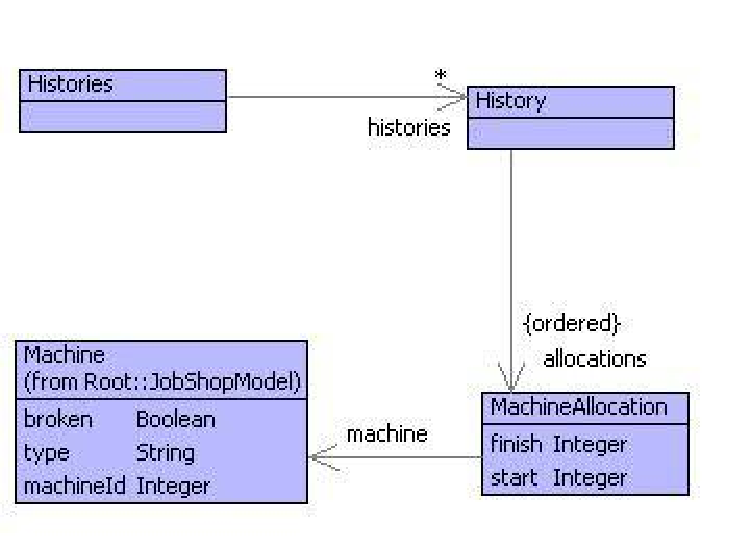
\includegraphics[width=8cm]{Programming/Simulation/Images/HistoryModels.pdf}

\caption{History Models\label{fig:History-Models}}

\end{center}
\end{figure}


An interesting analysis dertmines whether or not there are two jobs
that ever require the same machine at the same time. This analysis
requires a slightly diffferent type of simulation from that described
so far. In order to determine whether there may be a conflict, the
job shop is \emph{symbolically executed,} creating histories of possible
allocations of jobs to machines. These allocations can then be analysed
to determine whether any of them overlap.

Given the initial state of the job-shop it is possible to calculate
the scheduling options by analysing the plan for each job and allocating
the job to the machines it requires. The result of doing this for
each job is a collection of possible \emph{histories} for the simulation.
An execution of the simulation is represented by one possible history
for each of the jobs. If there is a machine that is required by two
different jobs in all possible histories then it is not possible to
optimally schedule the jobs, i.e. there is a bottleneck arising from
a conflict.

Consider the ProcessAircraft example given in a previous section.
Here are all the histories calculated for the jobs:

\begin{lstlisting}
Histories calculated for job Wing1:
  Option:
     Machine 3 is used from 0 to 5
     Machine 4 is used from 5 to 13
     Machine 5 is used from 13 to 16
  Option:
     Machine 3 is used from 0 to 5
     Machine 4 is used from 5 to 13
     Machine 6 is used from 13 to 16
  Option:
     Machine 3 is used from 0 to 5
     Machine 2 is used from 5 to 13
     Machine 6 is used from 13 to 16
  Option:
     Machine 3 is used from 0 to 5
     Machine 2 is used from 5 to 13
     Machine 5 is used from 13 to 16
Histories calculated for job Tail1:
  Option:
     Machine 3 is used from 0 to 5
     Machine 4 is used from 5 to 13
     Machine 5 is used from 13 to 16
  Option:
     Machine 3 is used from 0 to 5
     Machine 4 is used from 5 to 13
     Machine 6 is used from 13 to 16
  Option:
     Machine 3 is used from 0 to 5
     Machine 2 is used from 5 to 13
     Machine 6 is used from 13 to 16
  Option:
     Machine 3 is used from 0 to 5
     Machine 2 is used from 5 to 13
     Machine 5 is used from 13 to 16
Histories calculated for job Tail2:
  Option:
     Machine 3 is used from 0 to 5
     Machine 4 is used from 5 to 13
     Machine 5 is used from 13 to 16
  Option:
     Machine 3 is used from 0 to 5
     Machine 4 is used from 5 to 13
     Machine 6 is used from 13 to 16
  Option:
     Machine 3 is used from 0 to 5
     Machine 2 is used from 5 to 13
     Machine 6 is used from 13 to 16
  Option:
     Machine 3 is used from 0 to 5
     Machine 2 is used from 5 to 13
     Machine 5 is used from 13 to 16
Histories calculated for job Nose:
  Option:
     Machine 3 is used from 0 to 5
     Machine 4 is used from 5 to 13
     Machine 5 is used from 13 to 16
  Option:
     Machine 3 is used from 0 to 5
     Machine 4 is used from 5 to 13
     Machine 6 is used from 13 to 16
  Option:
     Machine 3 is used from 0 to 5
     Machine 2 is used from 5 to 13
     Machine 6 is used from 13 to 16
  Option:
     Machine 3 is used from 0 to 5
     Machine 2 is used from 5 to 13
     Machine 5 is used from 13 to 16
\end{lstlisting}Figure \ref{fig:History-Models} shows a model of job-shop histories.
A history records when a machine is busy in terms of when a job is
allocated to the machine (the start time) and when a job is removed
from the machine (the finish time). A job-shop is translated to an
instance of the class Histories, by calculating all the possible sets
of histories; each history is an ordered collection of consistent
machine allocations.

Each plan produces n instance of Histories:

\begin{lstlisting}
context Plan
  @Operation histories(jobShop)
    let h = Histories()
    in @For state in states do
         let M = jobShop.machines()->select(machine | 
                   machine.type() = state.machineType())
         in h.addMachines(state.duration(),M)
         end
       end;
       h
    end
  end
\end{lstlisting}A histories, adds all the machines that could occur during a given
time duration. The histories are built up incrementally by adding
machines that might be used by process descriptors. Since scheduling
is opportunistic each machine is allocated at random:

\begin{lstlisting}
context Histories
  @Operation addMachines(duration,M)
    // Add all the machines for the given duration at the
    // end of the current histories.
    @For history in histories do
      self.deleteFromHistories(history);
      @For machine in M do
        self.addToHistories(history.extend(duration,machine))
      end
    end
  end
\end{lstlisting}\begin{lstlisting}
context History
  @Operation extend(duration,machine)
    // Add a new allocation. Returns a copy so that
    // other additions don't interfere...
    let newHistory = self.copy();
        d = allocations->iterate(a d = 0 | d + (a.finish() - a.start()))
    in newHistory.addToAllocations(MachineAllocation(d,d + duration,machine))
    end
  end
\end{lstlisting}Two machine allocations conflict when they overlap:

\begin{lstlisting}
context MachineAllocation
  @Operation conflict(other:MachineAllocation):Boolean
    machine = other.machine and
    ((start >= other.start and start <= other.finish) or
     (other.start >= start and other.start <= finish))
  end
\end{lstlisting}Finally, the job-shop configuration has a conflict when there are
two jobs that require the same machine during the same time interval
in all possible histories:

\begin{lstlisting}
context JobShop
  @Operation conflict():Boolean
    jobs->exists(j1 |
      jobs->exists(j2 |
        j1 <> j2 and
        j1.plan().histories(self).histories()->forAll(h1 |
          j2.plan().histories(self).histories()->forAll(h2 |
            h1.allocations()->exists(a1 |
              h2.allocations()->exists(a2 | a1.conflict(a2)))))))
  end
\end{lstlisting}
